\newpage
\begin{center}
\noindent\textbf{ГЛАВА 1. РАСКРАСКИ СФЕР}\label{chapters:1}
\vspace{1.5mm}
\end{center}

\vspace{5pt}
\textbf{1.1 Постановка задачи и известные результаты}\label{chapters:1.1}
\vspace{5pt}

Графом называется пара $G=(V,~E)$, где $V$ - вершины графа, $E \subseteq \{\, (u,v) \mid u,v \in V \,\}$ - ребра графа. 
Хроматическим числом графа $\chi(G)$ называется минимальное число $k$ такое, что множество вершин $V$ можно разбить (покрасить) на $k$ 
непересекающихся классов $V_1 \sqcup V_1 \sqcup \dots \sqcup V_k = V$ так, что никакое ребро из $E$ не соединяет вершины одного класса. 
В данной работе рассматривается задача о хроматическом числе двумерной сферы 
$S^2(r) = \{\, x \in \mathbb{R}^3 : \|x\| = r \,\}$, сформулированная Полом Эрдёшем в 1981 году [\ref{bib:ErdosGraham}].
Предполагается, что расстояние между точками сферы $x,y \in S^2(r)$ задано евклидовой метрикой в $\mathbb{R}^3$: 
$d(x,y) = \sqrt{\sum_{i=1}^{3}(x_i-y_i)^2}$. Тогда 
$\chi(S^2(r)) = \min \{\, k: S^2(r) = V_1 \sqcup \dots \sqcup V_k , \, x,y \in V_i \Rightarrow \|x - y\| \ne 1 \,\}$. 
Во всех случаях, когда требуются непосредственные вычисления, предполагается, что центр сферы находится в начале координат.

Очевидно, что $\chi(S^2(r))$ зависит от $r$: если $r < \tfrac{1}{2}$, то $\chi(S^2(r))=1$, в то же время 
$S^2\left(\tfrac{1}{2}\right) = 2$ (подходит любая раскраска, в которой диаметрально противоположные точки имеют разный цвет).
При $r > \tfrac{1}{2}$ выполнено $\chi(S^2(r))>2$, так как соответствующий континуальный граф $G(S^2(r); 1)$ содержит нечетный цикл, для раскраски которого необходимы по крайней мере $3$ цвета.
В статье [\ref{bib:Simmons}] Симмонса был получен следующий результат:

\begin{theorem1}[Симмонс, 1976]
$$ \chi\left(S^2\left(\frac{1}{\sqrt{2}}\right)\right)=4, \quad \chi(S^2(r)) \geq 4 \text{ при } r > \frac{1}{\sqrt{3}}. $$
\end{theorem1}

Последнее неравенство было получено вложением в сферу конструкции, аналогичной \enquote{свернутому} веретену Мозера (\figurename{ \ref{chapter1:fig:simmons}}), для раскраски которой необходимо $4$ цвета. 
Отметим, что раскраска сферы $\chi\left(S^2\left(\frac{1}{\sqrt{2}}\right)\right)$ возникает в некой задаче квантовой механики, вследствие чего этот результат был переоткрыт другими авторами. Случай интересен тем, что $d(u,v)=1$ эквивалентно $(u,v)=0$ .
Из неравенства $\chi(\mathbb{R}^3) \leq 15$ следует, что 
$$\forall r>0 \quad \chi(S^2(r)) \leq 15.$$

\begin{figure}[h]
\centering
\captionsetup{justification=centering}
\begin{minipage}[h]{0.5\linewidth}
\center{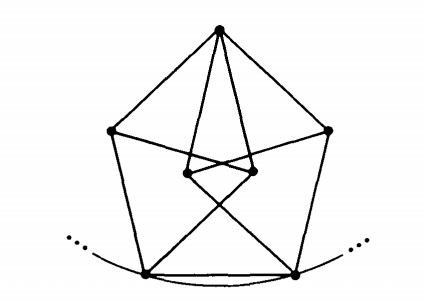
\includegraphics[width=0.4\paperwidth]{chapters/chapter1/simmons2.png}}
\end{minipage}\hfill
\begin{minipage}[h]{0.5\linewidth}
\center{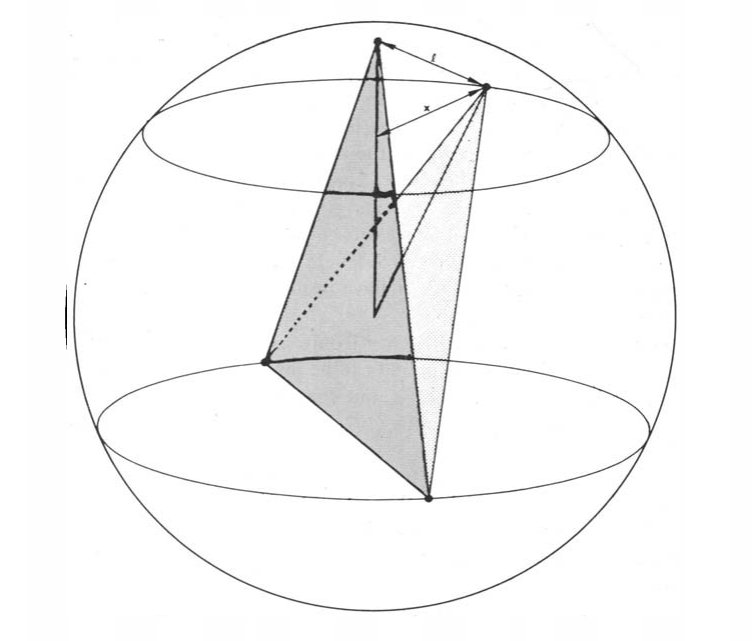
\includegraphics[width=0.4\paperwidth]{chapters/chapter1/simmons.png}}
\end{minipage}\hfill
\caption{К теореме Симмонса.}
\label{chapter1:fig:simmons}
\end{figure}

В дополнение к предыдущим рассмотрим некоторые асимптотические оценки и оценки для . В 1983 году  Л. Ловас доказал, что  $\chi(S^{n-1}(r)) \geq n$. В статье [\ref{bib:RaiSphere}] А.М. Райгородским показал, что хроматическое число сферы растет экспоненциально при росте размерности для всех $r > \frac{1}{2}$.

\begin{theorem1}

$$\text{Если } r \in (\frac{1}{2}, \frac{1}{\sqrt{2}}], \text{ то } 
\chi(S^{n-1}(r)) \geq \left(2(\frac{1}{8r^2})^{\frac{1}{8r^2}}(1-\frac{1}{8r^2})^{1-\frac{1}{8r^2}}+o(1)\right)^n.$$ 

$$\text{Если } r \geq \frac{1}{\sqrt{2}}, \text{ то } 
\chi(S^{n-1}(r)) \geq \left(2(\frac{1}{4})^{\frac{1}{4}}(\frac{3}{4})^{\frac{3}{4}}+o(1)\right)^n.$$

\end{theorem1}
В работе [\ref{bib:Kostina}] О. Костина доказала усиленный вариант предыдудщей теоремы.

\begin{theorem1}
Пусть $r > \tfrac{1}{2}$ и $b_1, b_{-1}$ таковы, что $b_1 + b_{-1} \in (0,1]$ и $b_1 < b_{-1}$.
Пусть $k_1=[b_1n]$ и $k_{-1}=[b_{-1}n]$. Положим

$$p_0(r,b_1,b_{-1},n) = \frac{(k_1 + k_{-1})n - (k_1 + k_{-1})^2}{2nr^2}$$
Пусть $p(r,b_1,b_{-1},n)$ - минимальное простое число, строго большее, чем $p_0$. 
Если при данных $r,b_1,b_{-1},n$ выполнено $k_1 + k_{-1} - 2p < -2k_{-1}$, то

$$\chi(S^{n-1}(r)) \geq 
\frac{\binom{n}{k_1}\binom{n-k_1}{k_{-1}}}
{\sum\limits_{(m_1,m_2) \, \in \, \mathcal{A}} \binom{n}{m_1} \binom{n-m_1}{m_2}}$$
где $\mathcal{A} = \{ (m_1,m_2): m_1,m_2 \in \mathbb{N} \cup \{ 0 \}, m_1+m_2 \leq n, m_1+2m_2 \leq p-1 \}$.

\end{theorem1}

Очевидно, что $\chi(S^{n-1}(r)) \leq \chi(\mathbb{R}^n) \leq (3+o(1))^n$, т.к. $S^{n-1}(r)$ лежит в $\mathbb{R}^n$. В общем случае лучших верхних оценок нет. Однако К.А. Роджерс [\ref{bib:Rogers}] получил более точную оценку в случае $r < \frac{3}{2}$.

\begin{theorem1}
$$\text{Если } r < \frac{3}{2}, \text{ то } \chi(S^{n-1}(r)) \leq (2r+o(1))^n.$$
\end{theorem1}

В работе [\ref{bib:Pros}] Р. Просановым получена следующая верхняя оценка хроматического числа сферы:

\begin{theorem1}
$\chi(S_r^{n-1}) \leq (x(r)+o(1))^n$, где
$$ x(r) = 
\begin{cases}
\sqrt{5-\frac{2}{r}+4\sqrt{1-\frac{5r^2-1}{4r^4}}},& \quad r > \frac{\sqrt{5}}{2} \\ 
2r,& \quad \frac{1}{2} < r \leq  \frac{\sqrt{5}}{2}
\end{cases}.$$
\end{theorem1}

Так как шестиугольники в раскраске плоскости (\figurename{ \ref{introduction:fig:plane}}) допускают небольшие деформации, кажется, что \enquote{почти плоский} участок сферы большого радиуса может быть раскрашен в $7$ цветов. Напрашивается заключение, что при достаточно большом $r$ в $7$ цветов может быть покрашена вся сфера, но на самом деле, как будет показано далее, аналогичных раскрасок всей сферы не существует. Тем не менее этот подход позволяет построить корректные 
раскраски сфер для некоторых диапазонов радиусов и получить на их основе верхние оценки для $\chi(S^2(r))$.

\vspace{5pt}
\textbf{1.2 Разбиение на области Вороного}\label{chapters:1.2}
\vspace{5pt}

Рассматриваются раскраски сферы $S^2(r)$ в $k$ цветов. Пусть $c(x)$  — цвет точки $x$, а $C_i$ — множество точек, раскрашенных в $i$-й цвет, $\bigcup\limits_{i=1}^{k} C_i = S^2(r)$. Требуется выполнить условие:

\begin{equation}\label{chapter1:propercoloring}
\forall \, x,y \in S^2(r), \, \|x - y\|=1 \Rightarrow c(x) \ne c(y)
\end{equation}

В данной работе в качестве таких одноцветных областей $C_i$ предлагается 
рассматривать выпуклые сферические многоугольники, построенные как области Ворон\textbf{о}го для некоторого набора точек.
Если задан набор точек (сайтов, генераторов) $x_1, x_2, \dots , x_m \in S^2(r)$, то диаграммой Вороного называется разбиение
$S^2(r)= \bigcup\limits_{i=1}^m V_i$, где $V_i$ - ячейки Вороного:
$$V_i = \{y \in S^2(r) \, : \quad \|y - x_j\| \geq \|y - x_i\|, \quad 1 \leq j \leq n, \, j \neq i \}.$$

Поскольку мы будем красить каждую область Вороного в один цвет, потребуем $\diam V_i < 1$, и, 
дополнительно, $\diam (V_i \bigcup V_j) > 1$, 
то есть мы не рассматриваем разбиение на области, которые могут быть объединены с соседними. 

В зависимости от контекста будем называть диаграммой Вороного как разбиение на ячейки, так и граф из вершин и ребер, составляющих эти ячейки. Такие мозайки названы в честь русского математика Георгия Вороного, который описал общий $n$-мерный случай в 1908 году,
являются фундаментальным инструментом вычислительной геометрии, широко используются в компьютерной графике, $3D$-моделировании, картографии, геофизике, химии, биологии. 
Для построения разбиений Вороного предложен ряд эффективных ($O(n\log{}n)$) алгоритмов и их компьютерных реализаций: 
\textit{CGAL}, \textit{TRIPACK}, \textit{STRIPACK}, \textit{Triangle}, \textit{QHull}, 
[\ref{bib:Larrea}], последний из которых является модификацией алгоритма Кларксона-Шора [\ref{bib:Barber}] и использовался в данной работе.

Мозайке Вороного однозначно соответствует граф триангуляции Делоне (состоящий из непересекающихся отрезков, соединяющий заданный набор точек так, что при построении плоскости через три точки, которые образуют треугольник, все остальные точки лежат не выше этой плоскости), который можно построить за $O(n)$:

\begin{theorem1}
Если соединить все сайты, соответствующие смежным ячейкам диаграммы Вороного, получится (двойственный) граф триангуляция Делоне для этого множества точек.
\end{theorem1}

\begin{figure}[h]
\centering
\captionsetup{justification=centering}
\center{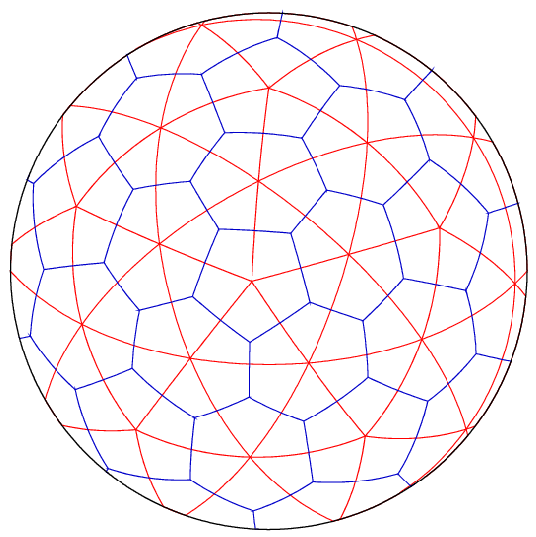
\includegraphics[width=0.3\paperwidth]{chapters/chapter1/triang-example.png}}
\caption{Диаграмма Вороного и двойственная триангуляция.}
\label{chapter1:fig:triangexample}
\end{figure}

На \figurename{ \ref{introduction:fig:plane}} приведен пример мозайки (синим) и двойственного графа.
Отметим, что для заданного набора точек сферическая триангуляция Делоне всегда существует, причём для каждого набора точек, в котором никакие четыре не лежат на одной окружности, она единственна.
Пусть задана набор точек и диаграмма Вороного. Обозначим как $\mathcal{G}$ граф триангуляции Делоне, двойственной к данной диаграмме. Предположим, что каждая из областей Вороного покрашена в некоторый цвет, и эта раскраска удовлетворяет условию 
(\ref{chapter1:propercoloring}). Раскрасим вершины $\mathcal{G}$ в цвета соответствующих областей. Тогда справедливы следующие утверждения.

\begin{statement}\label{chapter1:statement1}
Цвета смежных вершин $\mathcal{G}$ различны. 
\end{statement}

\begin{proof}
Предположим, что это неверно. Тогда объединение двух одноцветных областей имеет диаметр больше $1$, а поскольку это множество связно, то оно содержит и две одноцветные точки на единичном расстоянии, что противореит (\ref{chapter1:propercoloring}).
\end{proof}
 
\begin{statement}\label{chapter1:statement2}
Цвета вершин $\mathcal{G}$, находящихся на расстоянии $2$ (в смысле длины кратчайшего пути в графе), различны. 
\end{statement}

\begin{proof}
Поскольку диаметр любой области не превосходит единицы, расстояние между областями, имеющими общего соседа, меньше единицы,
значит найдется отрезок длины $1$, лежаший концами в этих областях. Следовательно, они должны иметь разные цвета.
\end{proof}

Пусть $\mathcal{G}^2$  — граф, в котором множество вершин совпадает с множеством вершин $\mathcal{G}$, 
а к ребрам из $\mathcal{G}$  добавлены ребра, соединяющие вершины, 
которые в графе $\mathcal{G}$ находились на расстоянии $2$:
$$E(\mathcal{G}^2) = \{ (u,v): \, (u,v) \in E(\mathcal{G}) \lor \exists \, w: \, (u,w),\,(w,v) \in E(\mathcal{G}) \}.$$
Тогда из построения $\mathcal{G}^2$ и утверждений 
\ref{chapter1:statement1} и \ref{chapter1:statement2} верно следующее.

\begin{statement}
Для существования правильной раскраски диаграммы Вороного в $k$ цветов необходимо, чтобы $\chi(\mathcal{G}^2) \leq k$.
\end{statement}

Если расстояние между $V_i$ и $V_j$, $i \neq j$ меньше единицы тогда и только тогда, 
когда соответствующие вершины смежны в $\mathcal{G}^2$, то последнее утверждение является необходимым и достаточным условием существования правильной раскраски сферы. Учитывая предыдещие построения и рассуждения, 
раскраску сферы в $k$ цветов получить из \enquote{подходящего} набора точек следующим образом: 
построить для них диаграмму Вороного, двойственный граф триангуляции $\mathcal{G}$, его квадрат $\mathcal{G}^2$, 
найти $k = \chi(\mathcal{G}^2)$, проверить выполнение всех необходимых условий и вычислить набор радиусов, 
при которых они выполняются. Если $d0$ - максимальный из диаметров областей $V_i$, $d1$ - минимальное из расстояний между областями на расстоянии $2$, то при выполнении всех остальных ограничений диапазон радиусов можно получить как 
$\left( \nicefrac{1}{d1}, \, \nicefrac{1}{d0} \right)$, где $\nicefrac{d1}{d0} < 1$.

Поиск хроматического числа графа является сам по себе сложной задачей. Для ее решения в данной работе использовались 
\textit{SAT}-решатели, которым посвящена вторая глава. Алгоритм поиска $\chi(G)$ вытекает из следующего утверждения.

\begin{statement1}\label{chapter1:formula}
Задача раскраски графа $G=(V,E)$ в $n$ цветов эквивалентна задаче булевой выполнимости формулы
$$F(G,n) = 
\bigwedge\limits_{v \in \textit{V}} 
\left( c_v^1 \vee \dots \vee c_v^n \right) 
\wedge 
\bigwedge\limits_{v \in \textit{V}, \, i < j \leq n } 
\left( \bar{c_v^i\vphantom{c_v^j}} \vee \bar{c_v^j} \right) 
\wedge 
\bigwedge\limits_{(v,w) \in \textit{E}, \, i \leq n} 
\left( \bar{c_v^i} \vee \bar{c_w^i} \right) \,,$$
где переменная $c_v^i$ равна $1$ тогда и только тогда, когда вершина $v$ покрашена в цвет $i$.
\end{statement1}

Вопросу о том, как получить подходящий набор точек-генераторов $\{ x_i \}$ посвящен следующий раздел.

\vspace{5pt}
\textbf{1.3 Задача Томсона}\label{chapters:1.3}
\vspace{5pt}

Множества точек $\{ x_i \}$, \textit{равномерно} распределенных на поверхности сферы, возникают как решения трудоемких задач многомерной оптимизации: задачи Томсона (о минимизации потенциала распределения точечных зарядов на сфере) и задачи о сферических кодах (максимизация минимального из попарных расстояний). 

Первая из задач сформулирована Дж. Дж. Томсоном в 1904 году [\ref{bib:Thomson}] при изучении \enquote{пудинговой} модели атома. 
Необходимо определить минимальную конфигурацию полной потенциальной энергии системы $N$ электронов, ограниченных поверхностью единичной сферы, которые отталкиваются друг от друга силой, определяемой Законом Кулона:

\begin{equation}\label{chapter1:thomson}
V(x_1, \dots, x_N) = \sum\limits_{i,j} \frac{1}{ \|x_i-x_j\| } \to \min\limits_{(x_1, \dots, x_N)}
\end{equation}

Cпустя век после постановки задача Томсона в трехмерном пространстве решена только для случаев 
$N = 2, 3, 4, 5, 6, 12$. 
При $N = 1$ решение тривиально. 
Два электрона располагаются в диаметрально противоположных точках.
Три электрона располагаются на большой окружности сферы в вершинах правильного треугольника.
Четыре электрона располагаются в вершинах правильного тетраэдра.
Для $N = 5$ в 2010 году было получено строгое компьютерное решение с электронами, находящимися в вершинах треугольной дипирамиды.
При $N = 6$ электроны находятся в вершинах правильного октаэдра.
При $N = 12$ электроны находятся в вершинах правильного икосаэдра.
При других $N$ экстремальность какой-либо конфигурации не доказана, 
однако для наших целей подходят и субоптимальные решения. Рассмотрим несколько алгоритмов их получения.

\textbf{Метод решетки} [\ref{bib:Altschuler}] позволяет получить расположение точек при $N = 10(m^2 + n^2 + mn) + 2$, 
где $m,n$ - целые числа, $N < 5000$. 
Пусть $\zeta = e^{\frac{i\pi}{3}}$, $\Delta$ - 
равносторонний треугольник с вершинами $0, m + \zeta n, \zeta m + \zeta^2 n$. Пересечение решетки $\Lambda$ с базисом $1, \zeta$ 
и треугольника $\Delta$ - конечное множество точек $\Delta$, которое отображается на грань вписанного в сферу икосаэдра. 
Остальные грани икосаэдра заполняются поворотом на $180^{\circ}$ относительно центра общего ребра соседних треугольников. 
Далее все полученные вершины радиально проецируются на поверхность сферы, после чего функционал суммарной энергии 
(\ref{chapter1:thomson}) оптимизируется методом сопряженных градиентов. 
$\upsilon_1(N)$ - количество целых чисел $l \le N$, для которых описанный алгоритм позволяет разместить электроны 
на поверхности сферы (существует решение соответствующего диофантова уровнения) можно грубо оценить как
$\upsilon_1(N) = 0.018N + 2.1\sqrt{N} + o(\sqrt{N})$.
На \figurename{ \ref{chapter1:fig:thomson}} приведен пример расположений зарядов для случаев $N=132$ (слева) и $N=1032$, полученных таким способом.

\begin{figure}[h]
\centering
\captionsetup{justification=centering}
\begin{minipage}[h]{0.5\linewidth}
\center{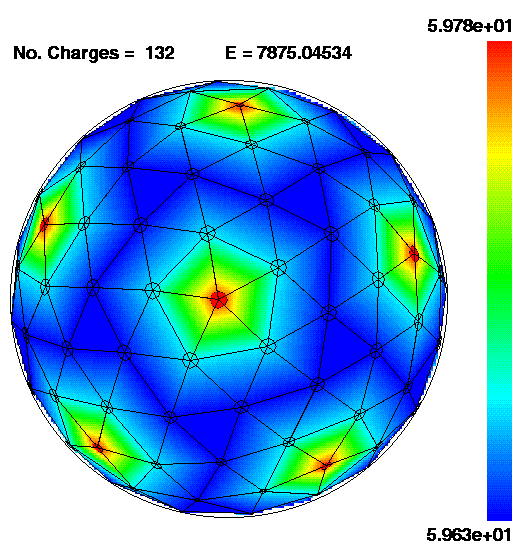
\includegraphics[width=0.35\paperwidth]{chapters/chapter1/thomson1.png}}
\end{minipage}\hfill
\begin{minipage}[h]{0.5\linewidth}
\center{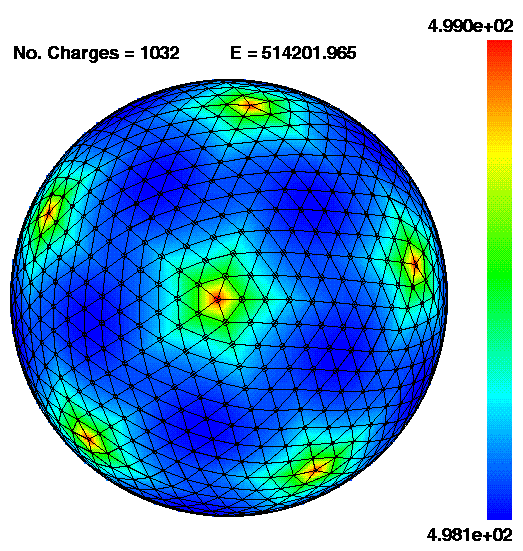
\includegraphics[width=0.35\paperwidth]{chapters/chapter1/thomson2.png}}
\end{minipage}\hfill
\caption{Субоптимальные решения задачи Томсона.}
\label{chapter1:fig:thomson}
\end{figure}

\textbf{Метод сечения икосаэдра} [\ref{bib:Katanforoush}] позволяет получить расположения лишь 
для $\upsilon_2(N) \simeq c\log{}N$ точек. 
Пусть $ABC$ - треугольник, и $a,\,b,\,c$ - середины его сторон $BC,\,CA,\,AB$. 
Тогда треугольник $abc$ разбивает $ABC$ на четыре треугольника (2-разрез). 
Такую операцию можно проделать для всех $20$ граней икосаэдра, 
получив триангуляцию из $80$ граней, $120$ ребер и $42$ вершин, радиальная проекция которой на сферу дает нужный результат. 
Аналогично строится $m$-разрез: каждая сторона треугольника делится на $m$ сегментов, порождая $m^2$ новых треугольников.
Эту операцию можно повторять итеративно, получая все более \enquote{мелкие} разбиения. 

Оба этих метода обладают полезным свойством. Назовем \textit{дефектом} вершины $\upsilon \in V(G)$ 
число $\delta(\upsilon) = 6 - deg(\upsilon)$. 
Тогда для графа триангуляции сферы $G$, построенного методом решетки или методом сечения икосаэдра выполнено 
$\sum\limits_{\upsilon_i \in V(G)} \delta(\upsilon_i) = 12$, что следует из построения и знаменитой формулы Эйлера для планарных графов: 
$v - e + f = 2$.
В частности, граф $G$ может содержать $12$ вершин степени $5$ и сколь угодно большое число вершин степени $6$. 
В дальнейшем будем рассматривать только такие графы. 

Решения, обладающие икосаэдральной симметрией, ($I$ в нотации Шeнфлиса) представляют особый теоретический интерес.
Их можно параметризовать парой натуральных чисел $p,q$ , где $p$ и $q$ - длины сторон параллелограмма на треугольной сетке, 
противоположные (острые) углы которого расположены в ближайших друг к другу вершинах степени $5$. 
Для графа при $N=132$ (\figurename{ \ref{chapter1:fig:thomson}}) $p=1,q=3$.
Cоответствующий граф будем обозначать $T(p,q)$. 
Некоторые теоретические оценки хроматических чисел для графов такого типа доказаны в третьей главе.

Для численных экспериментов в данной работе были использованы наилучшие 
известные на данный момент конфигурации зарядов для различных $N$, опубликованные 
в открытой коллекции решений различных оптимизационных задач Кембриджского университета
\textit{The Cambridge Cluster Database} [\ref{bib:Wales}]. 
Они получены различными способами, которые сводятся к выбору \enquote{хорошего} начального расположения
и дальнейшей оптимизации: 
используют градиентные методы, метод Монте-Карло, алгоритм имитации отжига, 
генетические алгоритмы, их комбинации и модификации [\ref{bib:Bondarenko}].

